

\tikzset{every picture/.style={line width=0.75pt}} %set default line width to 0.75pt        

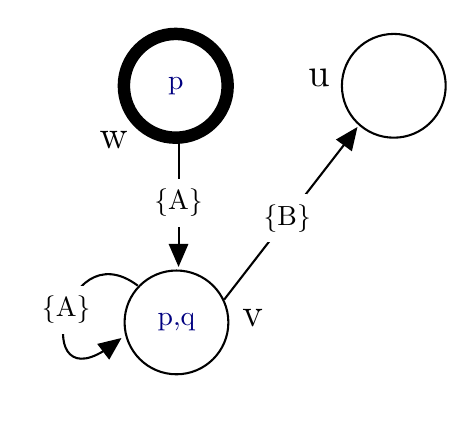
\begin{tikzpicture}[x=0.75pt,y=0.75pt,yscale=-1,xscale=1]
%uncomment if require: \path (0,300); %set diagram left start at 0, and has height of 300

%Straight Lines [id:da7382395640533164] 
\draw    (130.29,59) -- (130.29,118) ;
%Straight Lines [id:da018251469869151382] 
\draw    (152.29,135) -- (213,56.6) ;


%Shape: Circle [id:dp8938158972072578] 
\draw  [line width=0.75]  (104.29,146) .. controls (104.29,132.19) and (115.48,121) .. (129.29,121) .. controls (143.09,121) and (154.29,132.19) .. (154.29,146) .. controls (154.29,159.81) and (143.09,171) .. (129.29,171) .. controls (115.48,171) and (104.29,159.81) .. (104.29,146) -- cycle ;
%Shape: Circle [id:dp19780391712041556] 
\draw   (209,32) .. controls (209,18.19) and (220.19,7) .. (234,7) .. controls (247.81,7) and (259,18.19) .. (259,32) .. controls (259,45.81) and (247.81,57) .. (234,57) .. controls (220.19,57) and (209,45.81) .. (209,32) -- cycle ;
%Shape: Circle [id:dp06782137726568571] 
\draw  [line width=4.5]  (103.95,32) .. controls (103.95,18.19) and (115.15,7) .. (128.95,7) .. controls (142.76,7) and (153.95,18.19) .. (153.95,32) .. controls (153.95,45.81) and (142.76,57) .. (128.95,57) .. controls (115.15,57) and (103.95,45.81) .. (103.95,32) -- cycle ;
%Curve Lines [id:da0862450190271058] 
\draw    (110.62,128.27) .. controls (73.82,100.67) and (58.1,187.08) .. (98.1,157.08) ;

%Shape: Triangle [id:dp4725710951486233] 
\draw  [fill={rgb, 255:red, 0; green, 0; blue, 0 }  ,fill opacity=1 ] (101.8,154.28) -- (96.82,163.08) -- (91.97,156.67) -- cycle ;
%Shape: Triangle [id:dp08394946096129607] 
\draw  [fill={rgb, 255:red, 0; green, 0; blue, 0 }  ,fill opacity=1 ] (215.75,52.87) -- (213.48,62.72) -- (207.01,57.95) -- cycle ;

%Shape: Triangle [id:dp417855807516911] 
\draw  [fill={rgb, 255:red, 0; green, 0; blue, 0 }  ,fill opacity=1 ] (130.29,118) -- (126.27,108.72) -- (134.3,108.72) -- cycle ;


% Text Node
\draw (129.29,146) node  [align=left, NavyBlue] {p,q};
% Text Node
\draw (128.95,32) node  [align=left, NavyBlue] {p};
% Text Node
\draw  [color={rgb, 255:red, 255; green, 255; blue, 255 }  ,draw opacity=1 ][fill={rgb, 255:red, 255; green, 255; blue, 255 }  ,fill opacity=1 ]  (173.64,84.8) -- (191.64,84.8) -- (191.64,106.8) -- (173.64,106.8) -- cycle  ;
\draw (182.64,95.8) node  [align=left] {\{\agentSlide{B}\}};
% Text Node
\draw  [color={rgb, 255:red, 255; green, 255; blue, 255 }  ,draw opacity=1 ][fill={rgb, 255:red, 255; green, 255; blue, 255 }  ,fill opacity=1 ]  (67.14,129) -- (85.14,129) -- (85.14,151) -- (67.14,151) -- cycle  ;
\draw (76.14,140) node  [align=left] {\{\agentSlide{A}\}};
% Text Node
\draw  [color={rgb, 255:red, 255; green, 255; blue, 255 }  ,draw opacity=1 ][fill={rgb, 255:red, 255; green, 255; blue, 255 }  ,fill opacity=1 ]  (121.29,77.5) -- (139.29,77.5) -- (139.29,99.5) -- (121.29,99.5) -- cycle  ;
\draw (130.29,88.5) node  [align=left] {\{\agentSlide{A}\}};
% Text Node
\draw (99,58) node  [align=left] {\Large \poss{w}};
% Text Node
\draw (166,144) node  [align=left] {\Large \poss{v}};
% Text Node
\draw (198,28) node  [align=left] {\Large \poss{u}};


\end{tikzpicture}
